\documentclass{if-beamer}
\begin{document}
	
	\title[Campus Formoso do Araguaia]{Configuração de Redes e Servidores}
	\subtitle{Aula 4 }
	\author{Gilmar Gomes do Nascimento}
	\institute[IFTO]{
		Instituto Federal do Tocantins\\
		Campus Formoso do Araguaia
	}
	\date{\today}
	\logo{
		
\includegraphics[scale=0.0085]{logo.jpg}
	}
	\subject{Servers} % metadata
	
	\graphicspath{{figuras/}}
	%---------------------------------------------------------------------------------
	
	\begin{frame}
		\titlepage
	\end{frame}
	
	
    \begin{frame}[allowframebreaks]{Squid Proxy Server}
        \begin{figure}
            
\includegraphics[scale=.6]{squid-cache}
        \end{figure}
    \framebreak
    \begin{block}{Squid: Otimizando a entrega}
        Squid é um proxy de cache que suporta os protocolos HTTP, HTTPS, FTP e outros. Reduz 
        a largura de banda e melhora os tempos de resposta através do armazenamento em cache e 
        da reutilização de páginas frequentemente solicitadas. O Squid dispõe de controles de acesso
        abrangentes e constitui um excelente acelerador de servidores. Funciona na maioria dos
        sistemas operacionais, incluindo Microsoft Windows e é GNU GPL.
    \end{block}
    \framebreak

    \begin{block}{Aproveitando ao máximo sua conexão com a Internet}
        Squid é utilizado por centenas de fornecedores de serviços de Internet para otimizar
        o fluxo de dados entre o cliente e servidor, melhorando o desempenho e armazenamento 
        em cache de conteúdos utilizados com frequência para poupar largura de banda.		
    \end{block}

    \framebreak

    \begin{block}{Aceleração e distribuição de conteúdo}
        Milhares de sites utilizam o Squid para aumentar drasticamente a entrega dos conteúdos. 
        O Squid pode reduzir a carga e melhorar a velocidade de entrega aos clientes, copiando
        apenas os conteúdos que estão a ser utilizados, em vez de copiar tudo de forma ineficiente.

        Por fim, a configuração avançada de encaminhamento de conteúdos do Squid permite-lhe criar
        clusters de conteúdos para encaminhar e equilibrar a carga de pedidos através de uma variedade
        de servidores web.
    \end{block}			
    \end{frame}

    \begin{frame}{Por que usar Squid?}
        \begin{block}{Crescimento exponencial}
            Os criadores do protocolo HTTP identificaram o crescimento exponencial e, preocupados com o 
            mecanismo de distribuição, adicionaram poderosas primitivas de armazenamento em cache. 
            \begin{itemize}
                \item Validado
                \item Revalidado
                \item Armazenado
            \end{itemize}
        \end{block}
    \end{frame}
    
    \begin{frame}
        \begin{block}{Navegadores}
            As páginas são guardadas localmente para evitar consultas constantes à rede (especialmente úteis quando se navega por páginas estáticas)
        \end{block}
        \begin{block}{Redes de computadores}
            Por meio de um software que compartilha a conexão ou link, software este também chamado de proxy, que tem por função rotear as requisições
            a IPs externos à rede da qual faz parte. Os proxies têm capacidade de caching: ao armazenar o conteúdo de páginas web já visitadas pelos 
            usuários da rede na qual faz parte e fornecer esse conteúdo às novas requisições, minimizam o consumo da largura de banda e agilizam a
            navegação.				
        \end{block}
    \end{frame}
    \begin{frame}{Hands-on}
        \begin{enumerate}
            \item Instale o Squid-cache na máquina virtual
            \item Mostre-me as ações do serviço (squid)
            \item Configure para que não seja possível abrir nenhuma página com o domínio .bet na máquina virtual
        \end{enumerate}
    \end{frame}
    
\begin{frame}[allowframebreaks]{DNS}
	\begin{center}
		\Huge
		Domain Name Server (Sistema de nome de Domínios)
	\end{center}
	
	\framebreak 
		
	\begin{figure}
		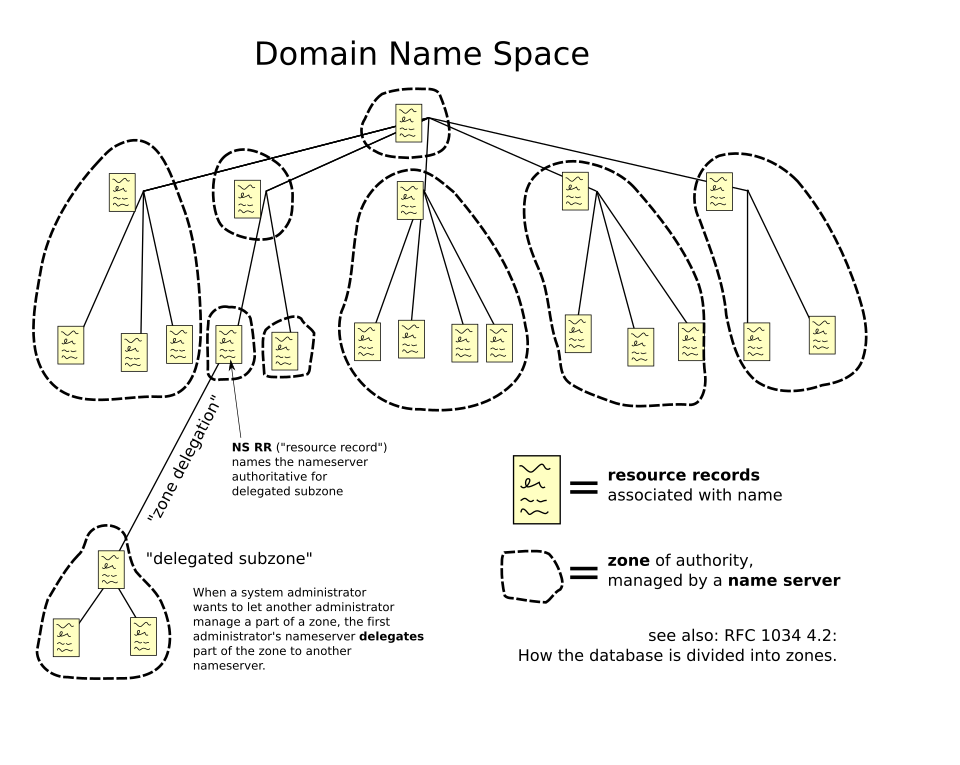
\includegraphics[scale=0.3]{dns}
	\end{figure}
	
\end{frame}
	
	\begin{frame}{Quatro servidores de DNS}
		\begin{itemize}
			\item Recursor de DNS
			\item Servidor Raiz
			\item Nameserver TLD
			\item Nameserver Autoritativo
		\end{itemize}
	\end{frame}
	
	\begin{frame}{Recurso de DNS}
	O recursor pode ser imaginado como um bibliotecário solicitado a procurar um livro específico em algum lugar de uma biblioteca. O recursor de DNS é um servidor projetado para receber consultas de máquinas clientes por meio de aplicativos como navegadores web. De modo geral, o recursor é responsável por fazer solicitações adicionais para atender à consulta de DNS do cliente.
	\end{frame}
%	
%	\framebreak
%	
	\begin{frame}{Servidor Raiz}
		é a primeira etapa da tradução (resolução) de host names legíveis por humanos em endereços de IP. Pode ser imaginado como um índice em uma biblioteca que aponta para diferentes estantes de livros, geralmente serve como referência para outros locais mais específicos.
	\end{frame}
%
%	\framebreak
%	
	\begin{frame}{Nameserver TLD}
		 Pense no servidor de domínio de nível superior (TLD) como uma estante de livros específica em uma biblioteca. Esse nameserver é o próximo passo na busca de um endereço de IP específico e hospeda a última parte de um hostname (em example.com, o servidor de TLD é ``com").
	\end{frame}
%	
%	\framebreak
%	
	\begin{frame}{Nameserver Autoritativo}
		 Pode ser imaginado como um dicionário em uma estante de livros, no qual um nome específico pode ser traduzido em sua definição. O nameserver autoritativo é a última parada na consulta de um servidor de DNS. Se tiver acesso ao registro solicitado, o nameserver autoritativo retornará o endereço de IP do hostname solicitado de volta ao recursor de DNS (o bibliotecário) que fez a solicitação inicial.
	\end{frame}


\begin{frame}[allowframebreaks]{As etapas de uma pesquisa de DNS}

	\begin{enumerate}
		\item Um usuário digita ``example.com" ~em um navegador web; a consulta viaja para a internet e é recebida por um resolvedor de DNS recursivo.
		\item O resolvedor então consulta um nameserver raiz de DNS(.).
		\item O servidor raiz responde ao resolvedor com o endereço de um servidor de DNS de Domínio de Nível Superior (TLD) (como \texttt{.com} ou \texttt{.net}) que armazena as informações de seus domínios. Quando buscamos example.com, nossa solicitação é direcionada para o TLD .com.

	\framebreak
	
	\item A seguir, o resolvedor faz uma solicitação ao TLD \texttt{.com}.
	\item A seguir, o servidor de TLD responde com o endereço de IP do nameserver do domínio, \texttt{example.com}.
	\item Para finalizar, o resolvedor recursivo envia uma consulta ao nameserver do domínio.
	
	\framebreak 
	
	\item O endereço de IP de \texttt{example.com} é a seguir retornado ao resolvedor partindo do nameserver.
	\item Em seguida, o resolvedor de DNS responde ao navegador web com o endereço de IP do domínio solicitado inicialmente.
	
	\framebreak
	
	\item O navegador faz uma solicitação de HTTP para o endereço de IP.
	\item O servidor nesse IP retorna a página da internet que deverá ser renderizada no navegador (etapa 10).
	
\end{enumerate}

	\begin{figure}
		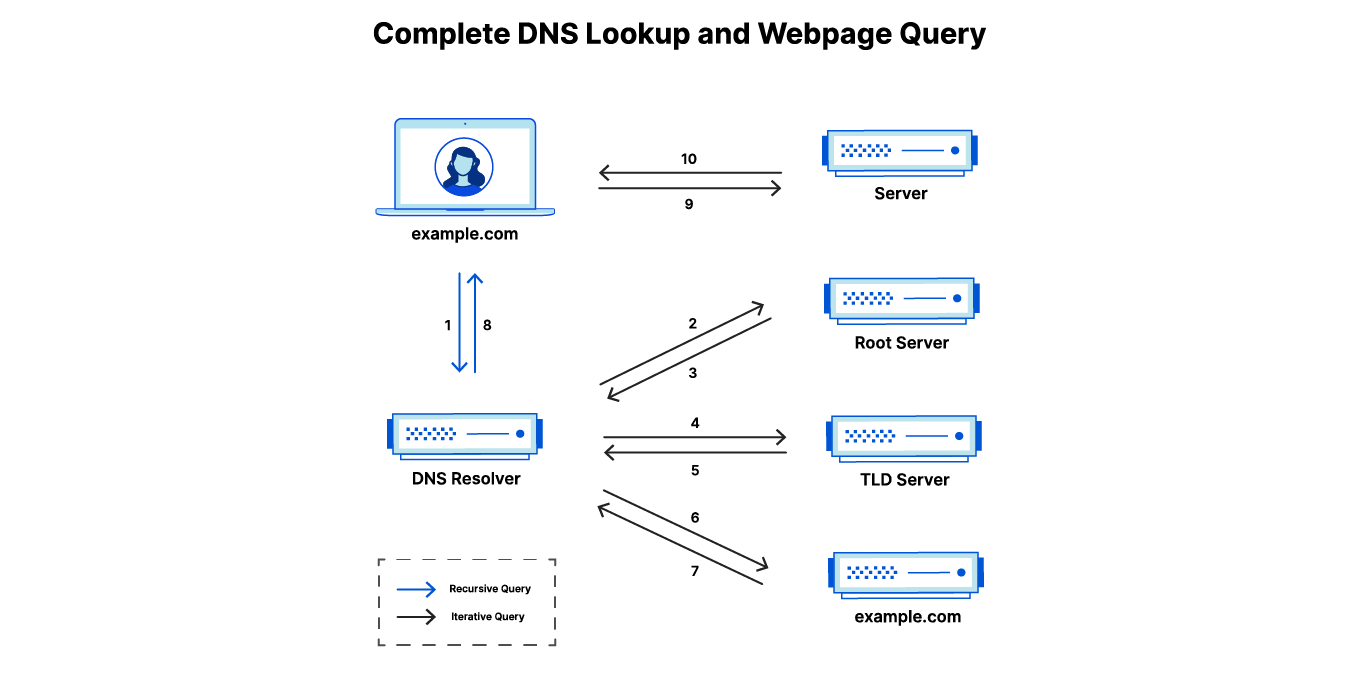
\includegraphics[scale=0.25]{complete-dns-lookup-and-webpage-query}
	\end{figure}
\end{frame}

\begin{frame}{Como descobrir qual DNS está sendo utilizado?}
	\centering
	\Huge
		\texttt{resolvectl status}
\end{frame}
    
 \begin{frame}{IPs de DNS público}
 	\begin{itemize}
 		\item \textbf{Google:} \texttt{8.8.8.8}~ \emph{e}~ ~\texttt{8.8.4.4}
 		\item \textbf{Cloudfare:} \texttt{1.1.1.1} ~ \emph{e}~ \texttt{1.0.0.1}
 		\item \textbf{Quad9:} \texttt{9.9.9.9} ~ \emph{e}~ \texttt{149.112.112.112}
 		\item \textbf{OpenDNS} \texttt{208.67.222.222} ~ \emph{e}~ \texttt{208.67.220.220}
 	\end{itemize}
 
 \end{frame}
 
 \begin{frame}[allowframebreaks]{Configuração do Squid}
 	\begin{itemize}
 		\item DNS
 		\item ACL
 		\item Regras de acesso
 		\item Configurações adicionais
 	\end{itemize} 
 
 	\framebreak
 	
 	\begin{exampleblock}{Ajustar permissões}
 	\large
 		\$ \\
 		\texttt{chown proxy:proxy /etc/squid/bloqueado.txt} \\
		\texttt{chmod 644 /etc/squid/bloqueado.txt}
	\end{exampleblock}
	
	\framebreak
	\begin{exampleblock}{Testar e configurar}
	\$ \\
		squid -k parse
	\end{exampleblock}
	\framebreak
	\begin{exampleblock}{Reiniciar o Squid}
		\centering
		\Large	
		\$ \\
			systemctl restart squid
	\end{exampleblock}
	
	\framebreak
	
	\begin{exampleblock}{Verificar status}
		\centering
			systemctl status squid
	\end{exampleblock}
	\begin{exampleblock}{Verificar se está escutando na porta 3128}
	\centering	
	netstat -tulpn | grep 3128
	\\ \emph{ou} \\
		ss -tulpn | grep 3128
	\end{exampleblock}
	
	\framebreak
	
	\begin{exampleblock}{Configurar o proxy no Navegador}
			\large
			\centering
				IP-DO-SERVIDOR \\
				PORTA: 3128
				
	\end{exampleblock}
 	\end{frame}
 	\begin{frame}{Outras ferramentas}
 	\begin{itemize}
 		\item \texttt{nslookup}
 		\item \texttt{dig}
 		\item \texttt{curl}
 		\item \texttt{hostname -I}
 	\end{itemize} 	
 	\end{frame}
 	
 	\begin{frame}{Bloqueado}
 		\begin{figure}
 			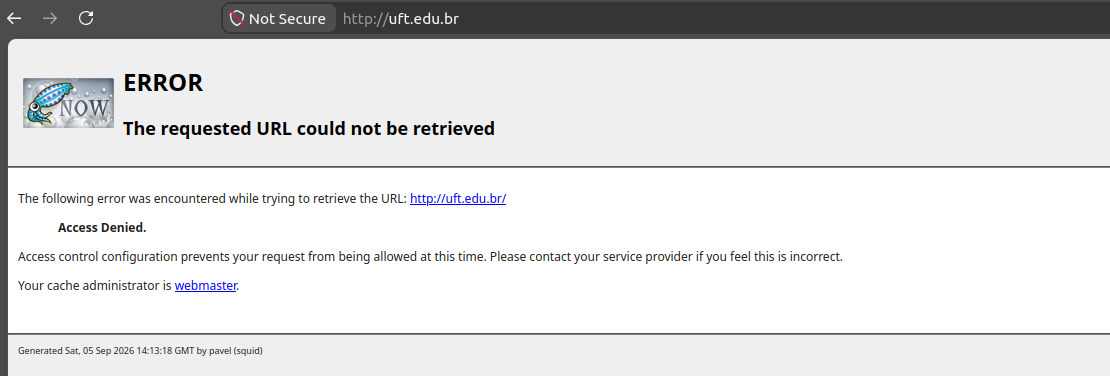
\includegraphics[scale=0.35]{bloqueado}
 		\end{figure}
 	
 	\end{frame}
 
 
% =========================================================
% NGINX
% ===========================================================
%
    \begin{frame}{NGINX}
        \begin{figure}
           
\includegraphics[scale=0.35]{nginx}
        \end{figure}
    \end{frame}   

    \begin{frame}{Nginx}

        \begin{quote}
            nginx (``engine x") is an HTTP web server, reverse proxy, content cache, load balancer, TCP/UDP proxy server, and mail proxy server. Originally 
            written by Igor Sysoev and distributed under the 2-clause BSD License. Enterprise distributions, commercial support and training are available from F5, Inc.
        \end{quote}
  \end{frame}
%    \framebreak
%
        \begin{frame}{Pré-requisitos}
            \texttt{sudo apt install curl gnupg2 ca-certificates lsb-release debian-archive-keyring -y} 
        \end{frame}
        
        \begin{frame}{Nginx}
        \Huge \centering
        	\texttt{nginx.org}
        
        \end{frame}
%        \begin{•}{Importar e autenticar chaves}
%            \texttt{curl https://nginx.org/keys/nginx_signing.key | gpg --dearmor \
%    | sudo tee /usr/share/keyrings/nginx-archive-keyring.gpg >/dev/null} 
%        \end{exampleblock}
%     \framebreak
%        \begin{exampleblock}{Verificar chaves}
%            \texttt{gpg --dry-run --quiet --no-keyring --import --import-options import-show /usr/share/keyrings/nginx-archive-keyring.gpg}
%        \end{exampleblock}
%    
 





    
% ============================================================
% REFERÊNCIAS
% ============================================================

\begin{frame}[allowframebreaks]{Referências}
	\begin{thebibliography}{9}
		
		\bibitem{cloudflare}
		Cloudflare	\textit{O que é DNS? | Como o DNS funciona}. Disponível em: \url{https://www.cloudflare.com/pt-br/learning/dns/what-is-dns/}. Acesso em: 8 set. 2026.
		\bibitem{heimdal}
		Heimdal \textit{TUDOR, Dora. Best free and public DNS servers}. Disponível em: \url{https://heimdalsecurity.com/blog/best-free-public-dns-servers}. Acesso em: 8 set. 2026.
		\bibitem{journald}
		Quad9. \textit{Quad9}. Disponível em: \url{https://quad9.net/pt/about/}. Acesso em: 26 de agosto de 2026.
		\bibitem{duckdns}
		Duck DNS. \textit{Duck DNS}. Disponível em: \url{https://www.duckdns.org/about.jsp}. Acesso em: 26 de agosto de 2026.
	
	\end{thebibliography}
\end{frame}	
\end{document}